\documentclass[10pt]{article}
\usepackage{sdss2020} % Uses Times Roman font (either newtx or times package)
\usepackage{url}
\usepackage{latexsym}
\usepackage{amsmath, amsthm, amsfonts}
\usepackage{algorithm, algorithmic}  
\usepackage{multirow,graphicx}
\usepackage[flushleft]{threeparttable}
\usepackage[T1]{fontenc}
\usepackage{booktabs}
\usepackage{siunitx} 
\usepackage[hidelinks]{hyperref}
\usepackage{supertabular}
\usepackage{xurl}
\usepackage{xcolor}
\usepackage{caption}

\graphicspath{ {./Images/} }
\newcolumntype{L}[1]{>{\raggedright\let\newline\\\arraybackslash\hspace{0pt}}m{#1}}
\newcolumntype{C}[1]{>{\centering\let\newline\\\arraybackslash\hspace{0pt}}m{#1}}
\newcolumntype{R}[1]{>{\raggedleft\let\newline\\\arraybackslash\hspace{0pt}}m{#1}}
\renewcommand{\thesubsection}{\thesection.\Alph{subsection}}
\renewcommand\fbox{\fcolorbox{gray}{white}}

\title{Modeling NHL Player Salaries: Evaluating Expectations}

\author{
  C. Logue \\
  Georgetown University \\
  Washington, DC \\
\\\And
  P. Mernagh \\
  Georgetown University \\
  Washington, DC \\
\\\And
  Z. Holden \\
  Georgetown University \\
  Washington, DC \\
\\}

\begin{document}
\maketitle

\section{Introduction}
The study aims to model NHL player salaries as a function of their key performance metrics. We are motivated by the availability of data around players’ offensive performance (e.g., shots, goals, and assists),  defensive performance (e.g., blocked shots and hits), position and team data points, and general demographic and physical characteristics. More advanced hockey statistics such as Corsi, Fenwick, shooting-plus-save percentage (PDO), and Expected Goals (xG) are also available for consideration. Since salaries are contractual and fixed before a season, we effectively evaluate players’ subsequent performance and determine whether they lived up to expectations. Though not dedicated hockey analysts, we have an initial understanding of potentially significant metrics that we wish to either confirm or invalidate. Our analysis accounts for some peculiarities of NHL finance, specifically entry-level contracts for rookies, but does not aim to capture the effects of signing bonuses, the salary cap, multi-year contracts, or players’ movements between the NHL and AHL. Nevertheless, we expect to discover key drivers of players’ salaries. 

\section{Data}
\subsection{Collection}
Our data was created by Rob Vallman, a former member of the Professional Hockey Writers Association, and an early author and blogger in the Hockey Analytics space. In 2017, Vallman publicly released a dataset with 154 season-level performance metrics for 874 players (non-goalies) in the prior NHL season (2016 - 2017). Vallman’s blog has long been taken down, but we were able to collect a redistribution of the data on Kaggle, an open-source data science platform which hosts datasets and competitions. 

\subsection{Cleaning}
The data upon receipt had been split into train and test sets; we begin by recombining. Player salaries are converted to millions of dollars, and the minimal number of null values are imputed with the median value of their respective columns. Outliers are identified but left alone. Players within the first three years of their NHL career are dropped, provided they are on fixed entry-level contracts that don’t appropriately reflect a club’s expectation. The players' years in the NHL (Yrs\_in\_NHL) are computed as 2016 - DftYr, their original draft year. As such, undrafted players are dropped, provided their contract form can’t be controlled for. Finally, we made the assumption that offensive players and defensive players would have fundamentally different expectations for their on-ice contribution. To hone our analysis, we decided to drop defensive players (Pos: D), instead opting to focus on offensive players (Pos: LW, RW, C). Our final cut was 382 hockey players.

\subsection{Summary Statistics}
Summary statistics for initially considered variables are found in \autoref{tab:summary_stats}. A complete data dictionary can be found in \autoref{a:data-dictionary}. 
\begin{table}[ht]
\caption{\label{tab:summary_stats}Summary Statistics (n =382)}
\centering
\begin{tabular}[t]{lrrr}
\toprule
  & mean & min & max\\
\midrule
Assists & 15.4 & 0.0 & 63.0\\
Corsi Against & 776.9 & 4.0 & 1678.0\\
Corsi For & 844.8 & 6.0 & 1983.0\\
Fenwick Against & 579.4 & 4.0 & 1264.0\\
Fenwick For & 629.8 & 5.0 & 1462.0\\
Faceoff Win Pct. & 41.2 & 0.0 & 100.0\\
Goals & 11.5 & 0.0 & 44.0\\
Goals Against & 36.0 & 0.0 & 91.0\\
Goals For & 40.7 & 0.0 & 120.0\\
Games Played & 57.7 & 1.0 & 82.0\\
Grit & 124.0 & 0.0 & 462.0\\
Height & 72.8 & 66.0 & 78.0\\
Blocks & 26.9 & 0.0 & 99.0\\
Hits Taken & 62.1 & 0.0 & 186.0\\
Hits Dished & 67.5 & 0.0 & 300.0\\
Shots & 105.0 & 0.0 & 313.0\\
PDO & 992.2 & 500.0 & 1257.0\\
Penalties in Min. & 28.5 & 0.0 & 133.0\\
Plus-Minus & -0.8 & -34.0 & 34.0\\
Salary & 2.9 & 0.6 & 14.0\\
Time on Ice & 52732.2 & 528.0 & 105263.0\\
Weight & 200.6 & 157.0 & 244.0\\
xG Against & 36.9 & 0.2 & 90.5\\
xG For & 41.5 & 0.1 & 111.1\\
Years in NHL & 8.7 & 4.0 & 26.0\\
\bottomrule
\end{tabular}
\end{table}


\section{Methods}
\subsection{Benchmark}
Our first objective is to construct a simple “baseline” model that can serve as a benchmark for alternative models. Fifteen features are carefully chosen along three dimensions we believe should be well-compensated: offensive production, defensive contribution, and overall physicality. The relationships between these covariates and the outcome of interest is explored. Pair plots exhibit positive, reasonably linear relationships between salary and the offensive covariates—Goals, Assists, Shots, Goals For, and Plus-Minus. Defensive covariates—Goals Against, Blocks, Hits, and Grit—show little to no relationship; while Years in the NHL, Height, Weight, Games Played and Time on Ice sit somewhere in the middle. Preliminary model fits demonstrate clear heteroscedasticity of residuals, along with non-normality characterized by heavy tails. Log transformation is applied to correct for this.
Multiple linear regression is fit, and residual diagnostics are performed. Variance Inflation Factors are estimated to formally evaluate multicollinearity. Finally, penalized methods are explored to perform model selection, as well as resolve multicollinearity. 

\subsection{Advanced Hockey Statistics}
In NHL analytics, “advanced” statistics are broadly defined as metrics that expand on the complexity of the traditional box-score statistics like goals, shots, hits, penalty minutes, or plus-minus differential. Traditional box-score statistics are typically combined with additional in-game measurements to provide a more nuanced understanding of how player performance—evaluated in terms of high-level concepts such as shot danger, quality of competition, and even “luck” (or lack thereof)—impacts key game outcomes. Their popularity has exploded in the past decade with in-house NHL franchise analytics departments to inform player contract offers, so we anticipate that their inclusion will increase the predictive power of the benchmark model. For simplicity in analysis, we choose to only consider the four fundamental advanced statistics, namely Corsi (C), Fenwick (F), expected goals (xG), and shooting-plus-save percentage (PDO).
To begin, we fit an initial saturated multiple linear regression model with the traditional box-score statistics from the benchmark model and the fundamental advanced statistics and perform residual and diagnostic analyses. Since advanced statistics are frequently considered together to provide complete context and cover blind spots from other metrics, we also incorporate interaction terms to capture established relationships between the offensive and defensive components of each advanced statistic, Corsi and Fenwick, and xG and PDO. There is significant overlap in the feature space among some of the advanced statistics—for example, Corsi and Fenwick both measure the sum of all shot attempts, except Fenwick excludes blocked shot attempts—so we apply a second round of LASSO penalized regression to perform model selection and resolve the reintroduced multicollinearity. 
Moreover, we observe noticeable heteroscedasticity in both the benchmark and advanced statistics models and therefore perform generalized least squares regression with both sets of covariates. Residual analysis demonstrates that this is likely caused by games played (\autoref{advanced-games}),
and we accordingly impose a heterogeneous variance pattern grouped by games played. The games are spaced at approximately equal intervals of time (excluding the mandatory mid-season bye week), and performance metrics are expected to serially correlate, as their increases and decreases usually happen together with slumps or streaks. Thus, we impose a first-order autoregressive, or AR(1), correlation pattern.


\subsection{GAM}
Since the benchmark model did not consider any nonlinear approaches, we finally assess whether any covariates can be appropriately modeled with a smoothed effect. We fit an initial GAM with REML and a smoother for every covariate, and perform residual and basis dimension diagnostics for each smoothed effect. We then fit a revised model, maintaining a smoothed effect for a small subset of the covariates. We also consider the case of dropping a potential outlier with respect to Years in the NHL.

\section{Results}
\subsection{Benchmark}
The initial OLS model %(\autoref{tab:initial} in \autoref{a:supplemental}) 
exhibits a strong degree of predictive power, with an adjusted coefficient of determination of 0.693. In residual analysis (\autoref{benchmark-residuals}), we observe a good degree of random scatter, with no trend in LOWESS that might suggest non-linearity in the regression function. Heteroscedasticity remains an issue, even with log transformation. There are no outliers. The QQ plot (\autoref{benchmark-qq}) exhibits normality, the result of an effective log transformation. Of the original fifteen covariates, the model shows strong evidence suggesting a linear relationship between Salary and only three—Time on Ice, Years in the NHL and Games Played. NHL career seems the most intuitive—for every year spent in the league, we observe a statistically significant increase in Salary by a factor of 1.06, or 6\%, on average, all else held equal. 
 In other words, there is a nice baseline “raise” for every year spent in the NHL. Beyond this, there are multiple signs of instability, of which many are recognized as informal signs of multicollinearity. In sensitivity analysis, many coefficients show large variation in both sign and magnitude—for example, when Goals is removed and the model re-fit, Assists flips to a positive factor, with Goals For cut in half. Strong, positive pairwise correlation is observed within the design matrix.
With a mean VIF = 14.91, there is strong evidence confirming influential collinearity in the predictors of interest; however, as we can observe in the individual VIF scores, multicollinearity is not consistently distributed among each covariates. Instead, correlation falls within stronger and weaker pockets of covariates, directly observable in the pairwise correlation plot—a stronger pocket emerges around offensive features, a slightly weaker among the defensive, and a little couplet around height and weight. Provided we have a high number of predictors, varying levels of importance and pockets of high correlation, we believe an elastic net is best-suited for penalized regression.
Elastic net is performed (\autoref{tab:benchmark}), showing a reasonably stable shrinkage. The lambda values are quite small, pointing to model selection as the best use case—we induce bias, but don’t observe any meaningful drop in the variance tradeoff. Iterating through different levels of $\alpha$, we settle on the traditional value at $\alpha = 0.5$, with the $\lambda$ chosen within the first standard error; introducing the $L_2$ norm to enforce a “grouping effect,” while leaning more heavily towards sparsity. Altogether, the model performs well along these expectations, preserving the group of offensive covariates, and shrinking out the unimportant group of defensive features, as we had expected might be the case. 
Comparing the shrinkage effect to the original OLS model (\autoref{tab:initial}), we observe correction in sign and magnitude that is perhaps more reasonable for interpretation. Assists are strongly corrected in the positive direction, and share similar impact to goals for—for every assist registered, we observe an increase in salary by a factor of about 1.1\%. This suggests that salary may be well-aligned with offensive production. Games played shrinks much closer to a neutral effect but remains negative. 

\begin{table}[ht]
\caption{\label{tab:benchmark}Benchmark Elastic Net}
\centering
\begin{threeparttable}
\begin{tabular}[t]{lc}
\toprule
 & s1 \\ 
  \midrule
(Intercept) & 0.2676 \\ 
  Goals & $\cdots$ \\ 
  Assists & 1.0107 \\ 
  Goals For & 1.0115  \\ 
  Goals Against & $\cdots$  \\ 
  Plus Minus & 0.9918 \\ 
  Time on Ice & 1.0000  \\ 
  Shots & 1.0022  \\ 
  Years in NHL & 1.0530 \\ 
  Height & $\cdots$ \\ 
  Weight & 1.0037 \\ 
  Hits Dished &  $\cdots$ \\ 
  Hits Taken &  $\cdots$ \\ 
  Blocks &  $\cdots$   \\ 
  Grit &  $\cdots$  \\ 
  Games Played & 0.9951 \\ 
\bottomrule
\end{tabular}
    \begin{tablenotes}
      \item $\alpha = 0.5, \lambda = 0.04$
    \end{tablenotes}
  \end{threeparttable}    
\end{table}

Ultimately, elastic net is effective, but doesn’t perfectly preserve groups—goals fall out of the offensive group, with height falling out of the physical characteristics grouping. To correct for this, we explored a penalized method called Group Lasso, introduced in 2006 for experiments in which a grouping of covariates is “natural.” The objective function is similar to Elastic Net in that it applies both the $L_1$ and $L_2$ norms; however, it first partitions the feature space by pre-defined “groupings,” and implements penalization separately within the subspaces. The model specification can be found in \autoref{tab:benchmark-grouped}. The model does correct the Elastic Net in preserving Goals and Height; however, the exponentiated coefficient estimates are inflated significantly. For the sake of reliability, we move forward with Elastic Net as our benchmark.  

\subsection{Advanced Hockey Statistics}
The initial multiple linear regression model with advanced statistics (\autoref{tab:advanced}) demonstrates improved predictive power over the benchmark model, achieving an adjusted coefficient of determination $R^2_a$ = 0.7161. In general, the interaction terms exhibit higher significance—measured in terms of p-value—than the underlying first-order covariates, which supports the modern conception of the four fundamental advanced statistics as starting metrics to drive compound analysis with other advanced statistics rather than meaningful metrics for independent analysis. That being said, our residual and diagnostic analyses indicate that it has two primary shortcomings that need to be remediated. 
First, the reintroduced multicollinearity is substantial, as indicated by the mean VIF = 182.6531, so we select a sparse representation of the model via LASSO regression (\autoref{tab:advanced-LASSO}), opting for the $L_1$ penalty corresponding to a cross-validated error within one standard error of the minimum given by $\lambda$ = 0.0151. Similar to the benchmark model, we find that this regularization largely favors the covariates closely related to offensive performance (e.g., team expected goals while the player was on the ice (xGF), team shot attempts while the player was on the ice (CF)) while shrinking the corresponding defensive components entirely out of the model.
Second, the heteroscedasticity observed in the residuals of the benchmark model conveys to the advanced statistics model (\autoref{advanced-residuals}), though the QQ plot still exhibits normality (\autoref{advanced-qq}). Accordingly, we perform GLS regression with both models (\autoref{tab:benchmark-gls} and \autoref{tab:advanced-gls} respectively), specifying the variance pattern as heterogeneous grouped by games played and the correlation pattern as first-order autoregressive. Plotting the standardized residuals against the fitted values for log-transformed salary, we find that the non-constancy of variance has been largely resolved in each case (\autoref{baseline-gls-residuals} and \autoref{advanced-gls-residuals} respectively). We then calculate the residual standard error ($se$) and Akaike information criterion for comparison, obtaining $se$ = 0.4217 and AIC = 709.1128 with the benchmark model and $se$ = 0.3266 and AIC = 693.7423 with the advanced statistics model. Thus, we conclude with certainty that the advanced statistics GLS regression model is superior to the benchmark GLS regression model in terms of both goodness-of-fit and parsimony.

\subsection{GAM}
Initial GAM results can be found in \autoref{tab.gam}%in \autoref{a:supplemental}
. A smoothed effect is modeled for Time on Ice, Years in the NHL, and Weight. Partial effect plots (\autoref{TOI-initial} - \autoref{Wt-initial}) demonstrate relatively good fit, with partial residuals falling fairly evenly around the smoothed function. However, the smoothed effect for Weight is still almost linear. Additionally, the smoothed effect for Years in the NHL is noticeably influenced in the right tail by an outlier, specifically Jaromír Jágr, who was drafted in 1990 and (as of writing) has had the longest career in professional ice hockey history. The revised GAM therefore only smooths Time on Ice and Years in the NHL, and considers the effect of dropping Jágr. Summarized results for the revised model are found in \autoref{tab.gam.revised}, with partial effect plots for Time on ice (\autoref{TOI-revised}) and Years in the NHL (\autoref{Yrs-in-NHL-revised}).  Deviance explained marginally decreases from 74.2\% to 73.9\%, but the Years in the NHL smoother is more justifiable. Significant covariates are similar between the initial and revised GAM vs. the benchmark model, with Time on Ice, Games Played, and Years in the NHL all highly significant. Concurvity analysis for both the initial and revised GAM models suggest room for improvement, similar to the multicollinearity in the benchmark model. High concurvity is seen in the offense-related covariates, and in Games Played and Time on Ice. Also similar to the benchmark model, the slightly negative Goals and Games Played coefficients are unintuitive and worth further remediation.

\section{Discussion}
Across the models considered, Assists, Goals, Shots, Time on Ice, Years in the NHL, and Games Played are generally significant. The defensive statistics we originally assumed predictive, namely Grit, Hits, and Blocks, were dropped in penalized regression, which is intuitive since we specifically modeled offensive players. We did attempt to model defensive players separately; even then, the defensive statistics were unexpectedly not very predictive. For both offensive and defensive players, Time on Ice, Years in the NHL, and Games Played remained significant.

It was not clear cut to identify or interpret the influence of team statistics on an individual player’s earnings. Goals For is significant, but by nature highly correlated with individual Goals. Plus-minus is also significant, and much less correlated with individual Goals. However, its negative coefficient is unexpected.

Additional data around player contracts, such as the form and length of entry-level contracts, the minimum salary, the team salary cap, and the typical length of multi-year contracts, would improve our modeling. Better understanding around games played, including data for games missed due to healthy scratches or to injury, as well as for  players sent down to the AHL, would aid with explanation. A more detailed data dictionary, with precise definitions and formulas for compound measures and the advanced hockey statistics, would help with interpreting their modeled effects. Finally, if we had data spanning multiple seasons, we could capture the effects of previous seasons on the renegotiation of a player’s contract. 

%\bibliographystyle{sdss2020} 
%\bibliography{bibl}

\section*{References}
\flushleft{DeMonte, D. (2020, May 6). \textit{Beginner’s Guide to Advanced Hockey Statistics}.
https://sites.northwestern.edu/nusportsanalytics/2020/05/06/\\advanced-hockey-statistics\\[1em]

\flushleft{Kaggle. (n.d.). \textit{Predict NHL Player Salaries}. 
https://www.kaggle.com/datasets/camnugent/predict-nhl-player-salaries/data\\[1em]

\flushleft{Vollman, R. (n.d.). \textit{NHL 2016-17 Player Data}.
https://web.archive.org/web/20171213112940/http://\\www.hockeyabstract.com/testimonials/nhl2016-17playerdata\\[1em]

\flushleft{Zlomislic, M. (2021, December 26). \textit{Hockey advanced analytics: What are they \& why are they important?}.
https://thehockeywriters.com/hockey-advanced-analytics-importance-metrics-definitions\\[1em]

\appendix
\clearpage

\section{Data Dictionary}
\label{a:data-dictionary}

\begin{table}[H]
\centering
%\caption*{Data Dictionary}
\label{data-dictionary}
\begin{tabular}[t]{p{0.2\columnwidth} p{0.7\columnwidth} }
\toprule
 & Meaning\\
\midrule
A & Assists, equivalent to A1 + A2\\
A1 & Primary assists\\
A2 & Secondary assists\\
CA & Shot attempts allowed (Corsi, SAT) while a player was on the ice\\
CF & The team's shot attempts (Corsi, SAT) while a player was on the ice\\
DftYr & Draft Year\\
FA & Unblocked shot attempts allowed (Fenwick, USAT) while a player was on the ice\\
FF & The team's unblocked shot attempts (Fenwick, USAT) while a player was on the ice\\
FO\_pct & Faceoff winning percentage \\
G & Goals\\
GA & Goals allowed while a player was on the ice\\
GF & The team's goals while a player was on the ice\\
GP & Games played\\
Grit & Hits, blocked shots, penalty minutes, and major penalties\\
Ht & Height, in inches\\
iBLK & Shots blocked\\
iHA & Hits taken\\
iHF & Hits thrown\\
iSF & Shots on goal\\
PIM & Penalties in minutes\\
plus\_mins & Plus/minus\\
TOI & Time on ice, in seconds\\
Wt & Weight, in pounds\\
xGA & Expected goals allowed (weighted shots) while a player was on the ice\\
xGF & The team's expected goals (weighted shots) while a player was on the ice\\
Yrs\_in\_NHL & Years in NHL (2016 - DftYr) \\
\bottomrule
\end{tabular}
\end{table}

\vfill\eject
\section{Supplemental Results}
\label{a:supplemental}

\begin{table}[tph]
\caption{Benchmark Model}
\label{tab:initial}
\centering
\begin{threeparttable}
\begin{tabular}[t]{lrrrr}
  \toprule
 & Estimate & t value & Pr($>$$|$t$|$) & 95\% CI \\ 
  \midrule
(Intercept) & 0.2862  & -1.142 & 0.254 & (0.0332, 2.4685) \\
  G & 0.9825 &  -2.004 & 0.046 & (0.9657, 0.9997) \\
  A & 0.9974 &  -0.346 & 0.729 & (0.9831, 1.0120) \\ 
  GF & 1.0145 &  2.562 & 0.011 & (1.0033, 1.0257) \\ 
  GA & 0.9939 & -1.305 & 0.193 & (0.9849, 1.0031) \\ 
  plus\_mins & 0.9907 &  -2.468 & 0.014 & (0.9833, 0.9981) \\ 
  TOI & 1.0000 &  4.812 &  $<$0.001 & (1.0000, 1.0000) \\
  iSF & 1.0024 & 2.166 & 0.031 & (1.0002, 1.0046) \\ 
  Years\_in\_ NHL & 1.0603 & 8.103 &  $<$0.001 & (1.0453, 1.0755) \\
  Ht & 0.9962 &  -0.196 & 0.844 & (0.9588, 1.0350) \\ 
  Wt & 1.0052  & 1.772 & 0.077 & (0.9994, 1.0109) \\ 
  iHF & 0.9995  & -0.278 & 0.781 & (0.9957, 1.0033) \\ 
  iHA & 1.0005  & 0.429 & 0.668 & (0.9981, 1.0030) \\ 
  iBLK & 0.9959  & -1.526 & 0.128 & (0.9908, 1.0012) \\ 
  Grit & 1.0013  & 0.916 & 0.360 & (0.9985, 1.0041) \\ 
  GP & 0.9740 & -7.210 & $<$0.001 &  (0.9670, 0.9810) \\ 
   \bottomrule
\end{tabular}
    \begin{tablenotes}
      \item $R^2_a$ = 0.69
    \end{tablenotes}
  \end{threeparttable} 
\end{table}

\begin{table}[tph]
\caption{\label{tab:benchmark-grouped}Benchmark Grouped LASSO}
\centering
\begin{threeparttable}
\begin{tabular}[t]{lc}
\toprule
 & s1 \\ 
  \midrule
(Intercept) & 1.9515\\ 
  Goals & 1.0597\\ 
  Assists & 1.2013 \\ 
  Goals For & 1.2367  \\ 
  Goals Against & $\cdots$ \\ 
  Plus Minus & 0.9236 \\ 
  Time on Ice & 1.1751 \\ 
  Shots & 1.1717  \\ 
  Years in NHL & 1.2207 \\ 
  Height & 1.0076 \\ 
  Weight & 1.0295 \\ 
  Hits Dished &  $\cdots$ \\ 
  Hits Taken &  $\cdots$ \\ 
  Blocks &  $\cdots$   \\ 
  Grit &  $\cdots$  \\ 
  Games Played & 0.8856 \\ 
\bottomrule
\end{tabular}
    \begin{tablenotes}
      \item $\lambda = 0.03$
    \end{tablenotes}
  \end{threeparttable}    
\end{table}

\begin{table}[tph]
\caption{Advanced Statisics Initial Model}
\label{tab:advanced}
\centering
\begin{threeparttable}
\begin{tabular}[t]{lrrrr}
  \toprule
  & Estimate & Std. Error & t value & Pr($>$$|$t$|$)\\
      \midrule
    (Intercept) & 0.2844 & 0.0682 & 4.17 & <0.0001 \\ 
    A & 0.0903 & 0.0871 & 1.04 & 0.3004 \\ 
    GF & 0.0835 & 0.2150 & 0.39 & 0.6978 \\ 
    Plus-Minus & -0.1309 & 0.0495 & -2.65 & 0.0085 \\ 
    TOI & 1.0859 & 0.3806 & 2.85 & 0.0046 \\ 
    iSF & 0.1505 & 0.0800 & 1.88 & 0.0608 \\ 
    Yrs\_in\_NHL & 0.2537 & 0.0293 & 8.65 & <0.0001 \\ 
    Wt & 0.0927 & 0.0292 & 3.17 & 0.0016 \\ 
    GP & -1.2380 & 0.1479 & -8.37 & <0.0001 \\ 
    PDO & 0.2387 & 0.1320 & 1.81 & 0.0714 \\ 
    CA & 1.2701 & 0.5870 & 2.16 & 0.0311 \\ 
    CF & 0.6446 & 0.7586 & 0.85 & 0.3961 \\
    FA & -1.0774 & 0.6302 & -1.71 & 0.0882 \\ 
    FF & 0.2472 & 0.8590 & 0.29 & 0.7737 \\ 
    xGA & -0.1335 & 0.2415 & -0.55 & 0.5807 \\ 
    xGF & -0.6520 & 0.3075 & -2.12 & 0.0347 \\ 
    CA:CF & -0.1448 & 0.4847 & -0.30 & 0.7653 \\ 
    FA:FF & 0.6112 & 0.5099 & 1.20 & 0.2314 \\ 
    CA:FA & -0.5539 & 0.1634 & -3.39 & 0.0008 \\ 
    CF:FF & -0.4170 & 0.1468 & -2.84 & 0.0047 \\ 
    xGA:xGF & 0.2437 & 0.1832 & 1.33 & 0.1842 \\ 
    PDO:xGA & 0.0339 & 0.1366 & 0.25 & 0.8040 \\ 
    PDO:xGF & 0.1089 & 0.1537 & 0.71 & 0.4789 \\ 
   \bottomrule
\end{tabular}
    \begin{tablenotes}
      \item $R^2_a$ = 0.72  % 0.7161, $df$ = 359, $se$ = 0.5328
    \end{tablenotes}
  \end{threeparttable}    
\end{table}

\begin{table}[tph]
\caption{\label{tab:advanced-LASSO}Advanced Statistics LASSO Model}
\centering
\begin{threeparttable}
   \begin{tabular}[t]{lr}
      \toprule
     & s1 \\
      \midrule
    (Intercept) & 0.0836 \\
    A & 0.0945 \\
    GF & 0.2345 \\
    plus\_mins & -0.0679 \\
    TOI & 0.1861 \\
    iSF & 0.1132 \\
    Yrs\_in\_NHL & 0.2367 \\
    Wt & 0.0678 \\
    GP & -0.4374 \\
    PDO & 0.0087 \\
    CA & $\cdots$ \\
    CF & 0.4549 \\
    FA & $\cdots$ \\
    FF & $\cdots$ \\
    xGA & $\cdots$ \\
    xGF & $\cdots$ \\
    CA:CF & $\cdots$ \\
    FA:FF & $\cdots$ \\
    CA:FA & -0.0309 \\
    CF:FF & -0.0530 \\
    xGA:xGF & $\cdots$ \\
    PDO:xGA & $\cdots$ \\
    PDO:xGF  & $\cdots$ \\
    \bottomrule
    \end{tabular}
    \begin{tablenotes}
      \item  $\alpha$ = 1, $\lambda$ = 0.0151
    \end{tablenotes}
  \end{threeparttable}    
\end{table}

\begin{table}[tph]
\caption{\label{tab:benchmark-gls}Benchmark GLS Model}
\centering
\begin{threeparttable}
\begin{tabular}[t]{lrrrr}
  \toprule
     & Estimate & Std. Error & t value & Pr($>$$|$t$|$) \\ 
  \midrule
    (Intercept) & -0.0620 & 0.0188 & -3.2835 & 0.0011 \\
    A & 0.0603 & 0.0589 & 1.0236 & 0.3067 \\
    GF & 0.3003 & 0.1033 & 2.9077 & 0.0039 \\
    Plus-Minus & -0.1223 & 0.0275 & -4.4414 & <0.0001 \\
    TOI & 0.9958 & 0.1175 & 8.4716 & $<$0.0001 \\
    iSF & 0.1042 & 0.0596 & 1.7469 & 0.0815 \\
    Yrs\_in\_NHL & 0.2384 & 0.0198 & 12.0294 & <0.0001\\
    Wt & 0.0570 & 0.0120 & 4.7497 & <0.0001 \\
    GP & -0.6863 & 0.0590 & -11.6330 & <0.0001\\
   \bottomrule
\end{tabular}
    \begin{tablenotes}
      \item AIC = 709.11
    \end{tablenotes}
  \end{threeparttable}    
\end{table}

\begin{table}[tph]
\caption{\label{tab:advanced-gls}Advanced Statistics GLS Model}
\centering
\begin{threeparttable}
\begin{tabular}[t]{lrrrr}
  \toprule
     & Estimate & Std. Error & t value & Pr($>$$|$t$|$) \\ 
  \midrule
    (Intercept) & 0.3141 & 0.0219 & 14.3129 & <0.0001\\
    A & 0.0488 & 0.0594 & 0.8226 & 0.4112 \\
    GF & 0.0817 & 0.1131 & 0.7224 & 0.4705 \\
    plus\_mins & -0.0552 & 0.0288 & -1.9138 & 0.0564 \\
    TOI & 1.1786 & 0.2429 & 4.8521 & $<$0.0001 \\
    iSF & 0.1678 & 0.0610 & 2.7482 & 0.0063 \\
    Yrs\_in\_NHL & 0.1959 & 0.0165 & 11.8570 & $<$0.0001 \\
    Wt & 0.0513 & 0.0142 & 3.6009 & 0.0004 \\
    GP & -1.3975 & 0.0585 & -23.8883 & $<$0.0001 \\
    PDO & 0.0007 & 0.0178 & 0.0421 & 0.9664 \\
    CA & 0.4754 & 0.3046 & 1.5607 & 0.1195 \\
    CF & 1.2594 & 0.4610 & 2.7318 & 0.0066 \\
    FA & -0.1993 & 0.3269 & -0.6097 & 0.5424 \\
    FF & -1.0619 & 0.4907 & -2.1636 & 0.0311 \\
    CA:FA & -0.3578 & 0.0304 & -11.7530 & $<$0.0001 \\
    CF:FF & 0.0136 & 0.0305 & 0.4460 & 0.6558 \\
   \bottomrule
\end{tabular}
    \begin{tablenotes}
      \item AIC = 693.74
    \end{tablenotes}
  \end{threeparttable}    
\end{table}


\begin{table}[tph]
\centering
\caption{Initial GAM} 
\label{tab.gam}
\begin{threeparttable}
\begin{tabular}[t]{L{0.27\linewidth}rrrr} 
   \toprule
A. parametric coefficients & Estimate & Std. Error & t-value & p-value \\ 
   \midrule
  (Intercept) & 0.6686 & 0.0246 & 27.2225 & $<$ 0.0001 \\ 
   \midrule
B. smooth terms & edf & Ref.df & F-value & p-value \\ 
   \midrule
  s(G) & 1.0001 & 1.0002 & 4.8506 & 0.0283 \\ 
  s(A) & 1.0000 & 1.0001 & 0.0048 & 0.9450 \\ 
  s(GF) & 1.0008 & 1.0014 & 6.2768 & 0.0126 \\ 
  s(plus\_mins) & 1.1457 & 1.2784 & 2.9811 & 0.0569 \\ 
  s(TOI) & 3.8517 & 4.8294 & 11.2133 & $<$ 0.0001 \\ 
  s(iSF) & 1.0000 & 1.0000 & 9.9730 & 0.0017 \\ 
  s(Yrs\_in\_NHL) & 3.2940 & 4.1439 & 25.0174 & $<$ 0.0001 \\ 
  s(Wt) & 2.0294 & 2.6114 & 5.0137 & 0.0031 \\ 
  s(GP) & 1.0000 & 1.0001 & 77.7958 & $<$ 0.0001 \\ 
   \bottomrule
\end{tabular}
    \begin{tablenotes}
      \item Deviance explained = 74.2\%
    \end{tablenotes}
  \end{threeparttable}    
\end{table}

\begin{table}[tph]
\centering
\caption{Revised GAM} 
\label{tab.gam.revised}
\begin{threeparttable}
%\scriptsize
\begin{tabular}[t]{L{0.27\linewidth}rrrr} 
   \toprule
A. parametric coefficients & Estimate & Std. Error & t-value & p-value \\  
  \midrule
  (Intercept) & 0.9463 & 0.4591 & 2.0612 & 0.0400 \\ 
  G & -0.0179 & 0.0081 & -2.2001 & 0.0284 \\ 
  A & 0.0008 & 0.0069 & 0.1100 & 0.9125 \\ 
  GF & 0.0130 & 0.0052 & 2.5194 & 0.0122 \\ 
  plus\_mins & -0.0061 & 0.0030 & -2.0545 & 0.0406 \\ 
  iSF & 0.0031 & 0.0010 & 3.1489 & 0.0018 \\ 
  Wt & 0.0066 & 0.0019 & 3.4912 & 0.0005 \\ 
  GP & -0.0393 & 0.0045 & -8.7432 & $<$ 0.0001 \\ 
   \midrule
B. smooth terms & edf & Ref.df & F-value & p-value \\ 
  \midrule
  s(TOI) & 3.8041 & 4.7758 & 11.0928 & $<$ 0.0001 \\ 
  s(Yrs\_in\_NHL) & 3.0052 & 3.7576 & 27.4259 & $<$ 0.0001 \\ 
   \bottomrule
\end{tabular}
    \begin{tablenotes}
     %\scriptsize
      \item Deviance explained = 73.9\%
    \end{tablenotes}
  \end{threeparttable}    
\end{table}

\vfill\break
\section{Supplemental Figures}
\label{a:supplemental-fig}

\begin{figure}[tph]
\centering
	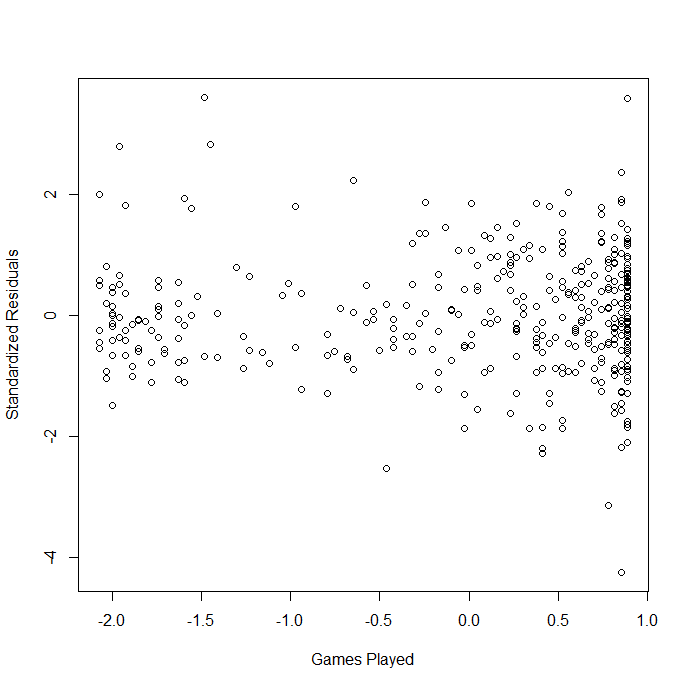
\includegraphics[width=0.9\columnwidth]{games_played_vs_resid_sq}
	\caption[]
    	{\tabular[t]{@{}l@{}}Standardized Residuals vs Games Played\endtabular}
	\label{advanced-games}
\end{figure}

\begin{figure}[tph]
\centering
	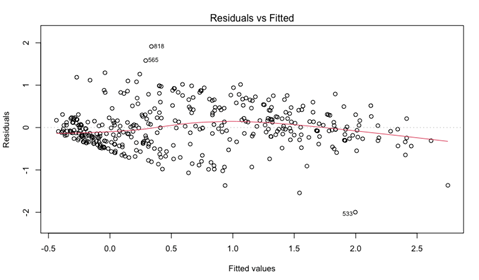
\includegraphics[width=0.9\columnwidth]{benchmark_residuals_vs_fitted}
	\caption[]
    	{\tabular[t]{@{}l@{}}Residuals vs. Fitted Plot (Benchmark)\endtabular}
	\label{benchmark-residuals}
\end{figure}

\begin{figure}[tph]
\centering
	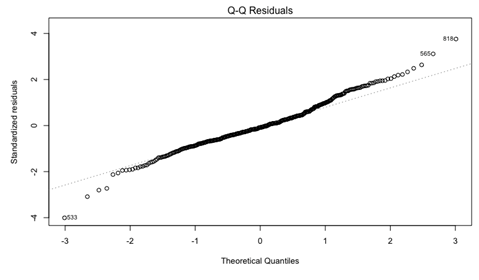
\includegraphics[width=0.9\columnwidth]{benchmark_qq}
	\caption[]
    	{\tabular[t]{@{}l@{}}Q-Q Plot (Benchmark)\endtabular}
	\label{benchmark-qq}
\end{figure}

\begin{figure}[tph]
\centering
	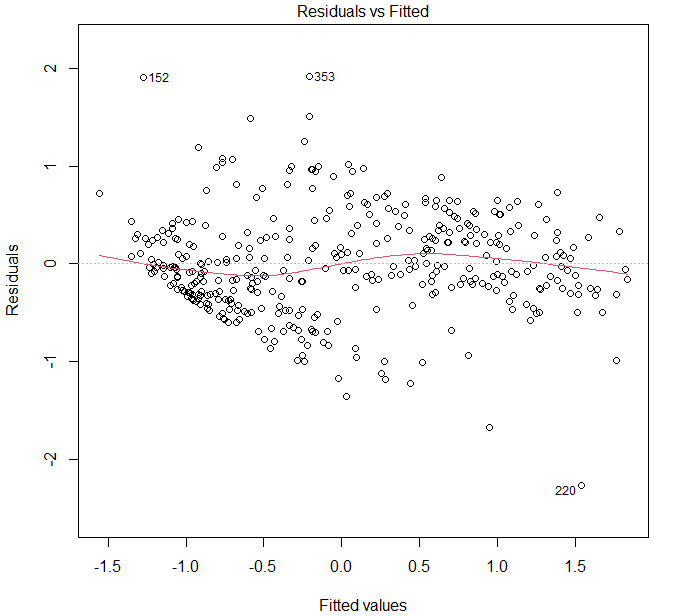
\includegraphics[width=0.9\columnwidth]{model_ols_adv_resid_vs_fitted_sq_adj}
	\caption[]
    	{\tabular[t]{@{}l@{}}Residuals vs. Fitted Plot \\(Advanced Statistics)\endtabular}
	\label{advanced-residuals}
\end{figure}

\begin{figure}[tph]
\centering
	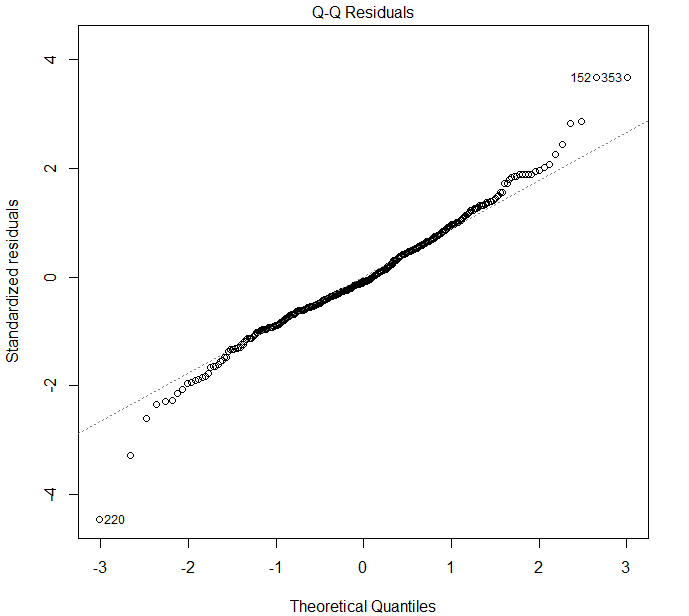
\includegraphics[width=0.9\columnwidth]{model_ols_adv_qq_resid_sq_adj}
	\caption[]
    	{\tabular[t]{@{}l@{}}Q-Q Plot (Advanced Statistics)\endtabular}
	\label{advanced-qq}
\end{figure}

\begin{figure}[tph]
\centering
	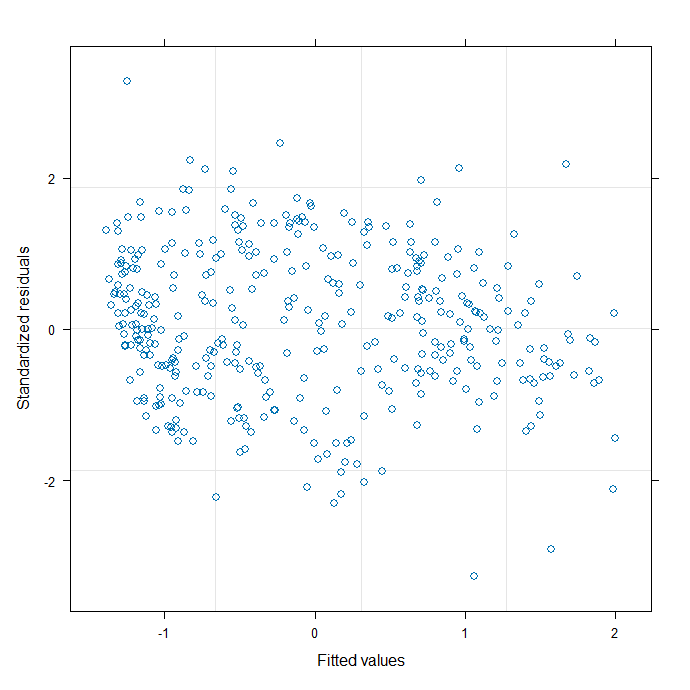
\includegraphics[width=0.9\columnwidth]{model_gls_base_resid_vs_fitted_sq}
	\caption[]
    	{\tabular[t]{@{}l@{}}Residuals vs. Fitted Plot\\(Baseline GLS)\endtabular}
	\label{baseline-gls-residuals}
\end{figure}

\begin{figure}[tph]
\centering
	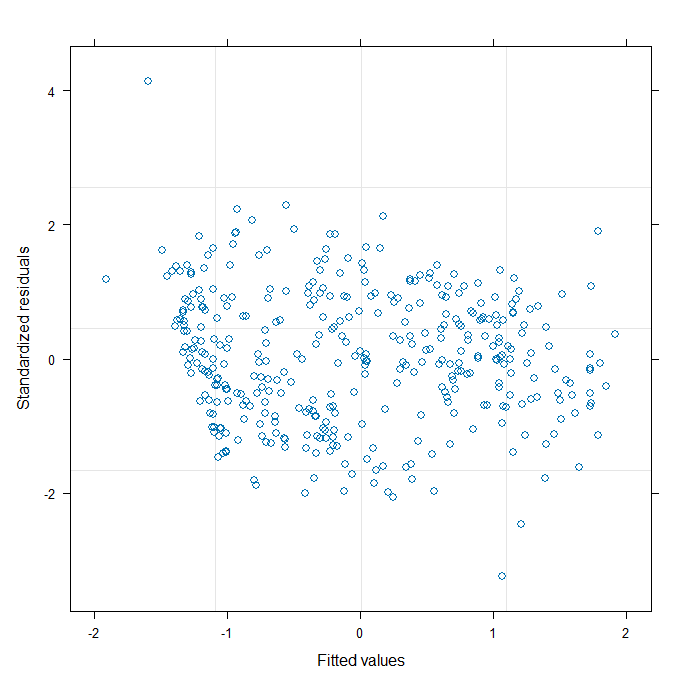
\includegraphics[width=0.9\columnwidth]{model_gls_adv_resid_vs_fitted_sq}
	\caption[]
    	{\tabular[t]{@{}l@{}}Residuals vs. Fitted Plot \\(Advanced Statistics GLS)\endtabular}
	\label{advanced-gls-residuals}
\end{figure}

\begin{figure}[tph]
\centering
	\fbox{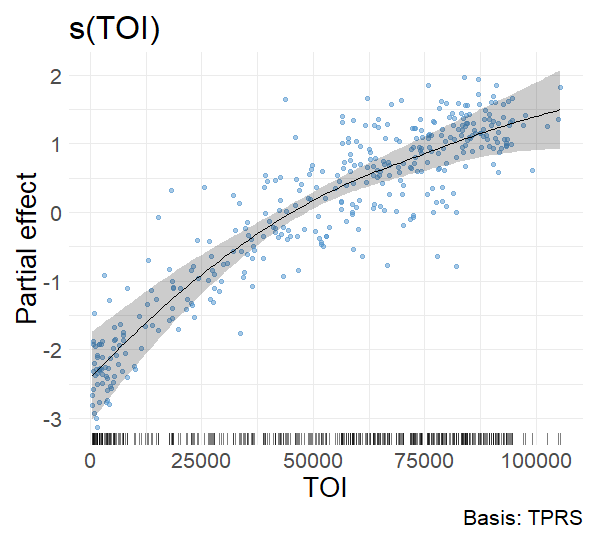
\includegraphics[scale=0.4]{s(TOI)}}
	\caption[]
    	{\tabular[t]{@{}l@{}}Partial Effects Plot, Time on Ice \\ (Initial GAM)\endtabular}
	\label{TOI-initial}
\end{figure}

\begin{figure}[tph]
\centering
	\fbox{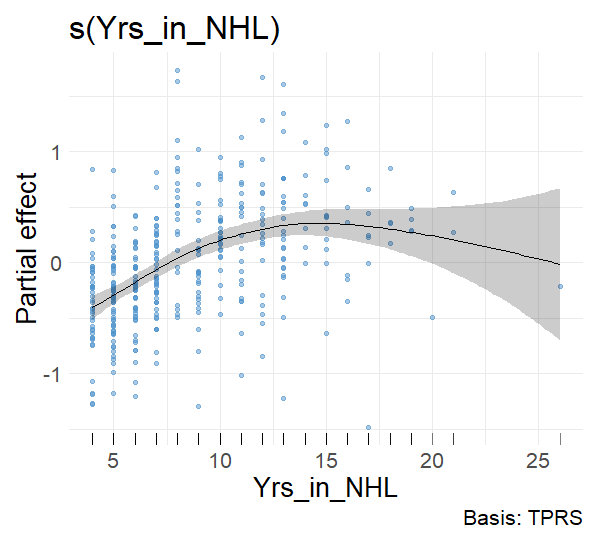
\includegraphics[scale=0.4]{s(Yrs_in_NHL)}}
	\caption[]
    	{\tabular[t]{@{}l@{}}Partial Effects Plot, Years in NHL \\ (Initial GAM)\endtabular}
	\label{Yrs-in-NHL-initial}
\end{figure}

\begin{figure}[tph]
\centering
	\fbox{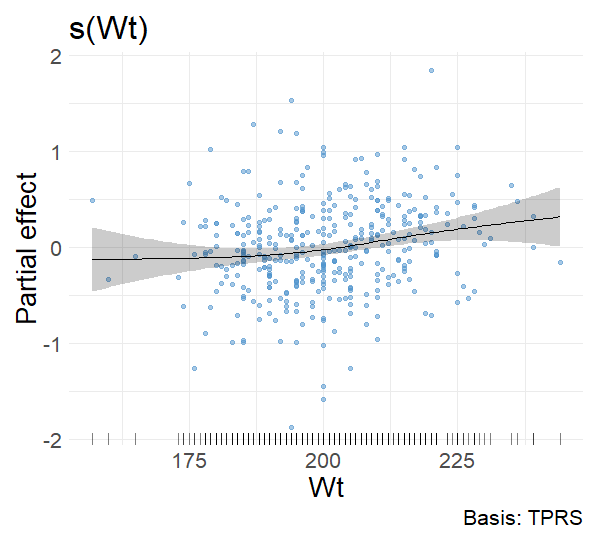
\includegraphics[scale=0.4]{s(Wt)}}
	\caption[]
    	{\tabular[t]{@{}l@{}}Partial Effects Plot, Weight \\ (Initial GAM)\endtabular}
	\label{Wt-initial}
\end{figure}

\begin{figure}[tph]
\centering
	\fbox{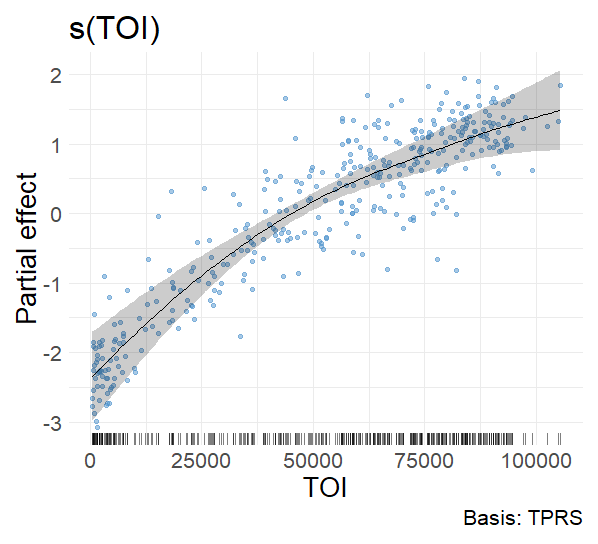
\includegraphics[scale=0.4]{s(TOI)_revised}}
	\caption[]
    	{\tabular[t]{@{}l@{}}Partial Effects Plot, Time on Ice \\ (Revised GAM)\endtabular}
	\label{TOI-revised}
\end{figure}

\begin{figure}[tph]
\centering
	\fbox{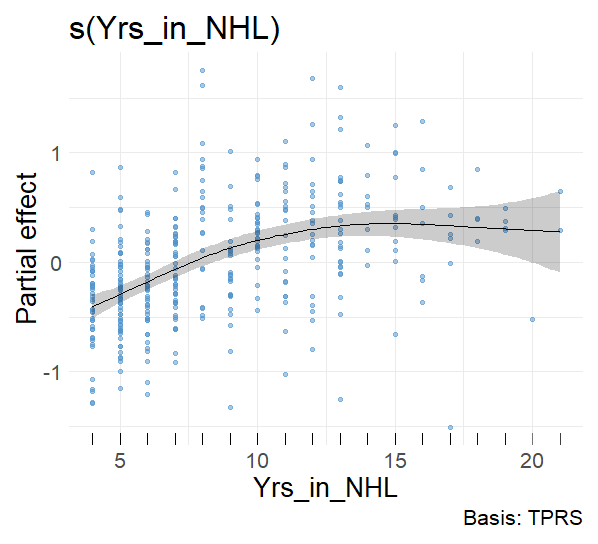
\includegraphics[scale=0.4]{s(Yrs_in_NHL)_revised}}
	\caption[]
    	{\tabular[t]{@{}l@{}}Partial Effects Plot, Years in NHL\\ (Revised GAM)\endtabular}
	\label{Yrs-in-NHL-revised}
\end{figure}

%\clearpage
\vfill\eject
\section{Replication Data and Code}
\label{a:code}
Replication data and code can be found in the GitHub repo \mbox{https://github.com/cons-code/MATH-5500}.

\end{document}